% kate: word-wrap true;

\chapter{Writing System}
\index{Tahano Hikamu|(}

In the past chapter, example words were given in Ayeri's script, \rayr{thno 
hikmu}{Tahano Hikamu}, wherever possible. Thus, it seems advisable to include a 
description of Ayeri's native writing system here as well. Literally, 
\rayr{thno hikmu}{Tahano Hikamu} means `Round Script' (script round), which is 
an old formation based on the word \xayr{thnF/}{tahan-}{write} that  stuck. The 
current word for `script' is \xayr{thnnF}{tahanan}{writing}. Tahano Hikamu was 
originally named thus because of an earlier draft for a script that never made 
it very far beyond the drawing board and which was a lot more angular, or 
\rayr{hinY}{hinya}, see \autoref{fig:hinya}.\footnote{Unfortunately, there is 
no documentation surviving that I know of.}\index{Tahano Hinya}

\begin{figure}[tp]
\caption{Tahano Hinya and Hikamu}

\begin{minipage}{.5\linewidth}
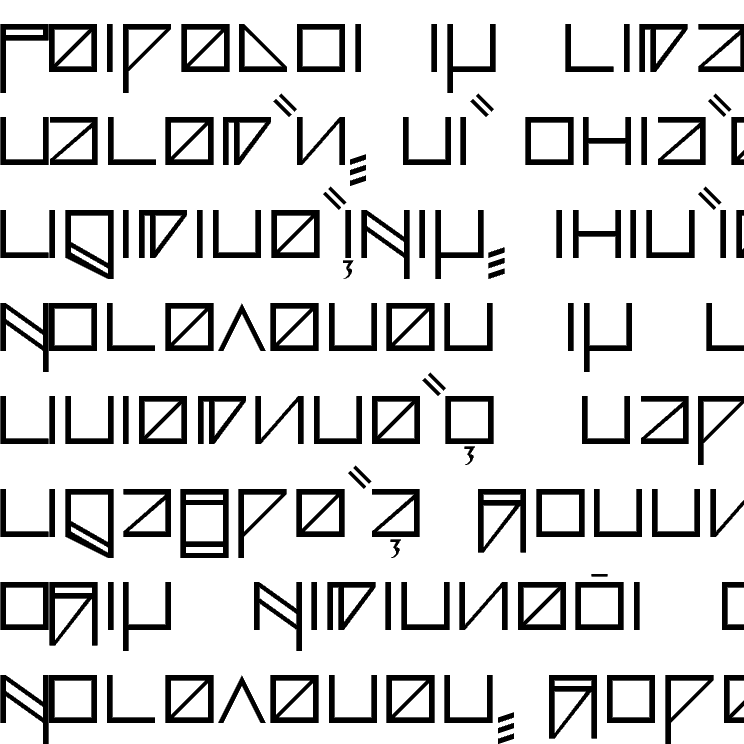
\includegraphics[width=\linewidth]{images/hinya-300dpi-clip.png}
\subcaption{Old and aborted draft: Tahano Hinya}
\label{fig:hinya}
\end{minipage}
~
\begin{minipage}{.5\linewidth}
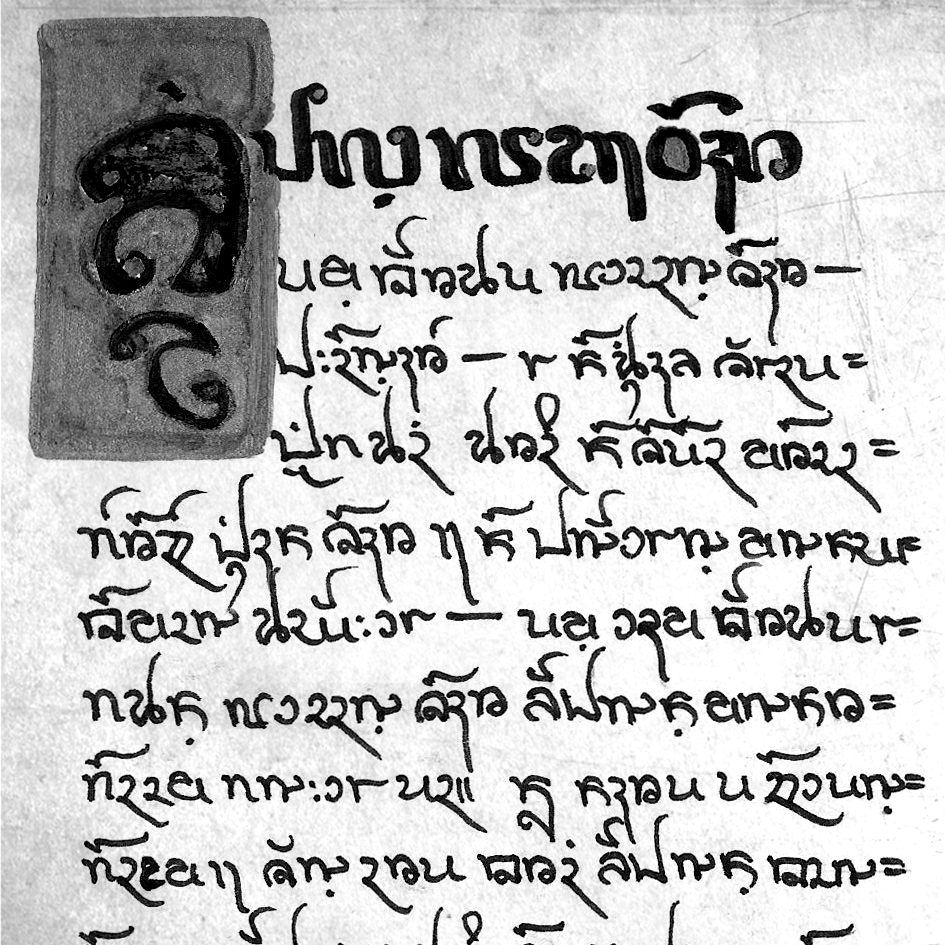
\includegraphics[width=\linewidth]{images/tahano-300dpi-bw-clip.png}
\subcaption{Ayeri's native script: Tahano Hikamu}
\end{minipage}

\label{fig:hinyahikamu}
\end{figure}

As we have seen in the previous chapter, Ayeri's prosody strongly emphasizes 
the syllable as a unit. Thus, it is not a surprise that Ayeri's native script,
Tahano Hikamu, is an alphasyllabary like the Brāhmī-derived alphabets of India 
and Southeast Asia \parencites{salomon1996}{court1996}.\index{Brāhmic scripts} 
This means that its 

\blockcquote[376]{salomon1996}{system is based on the unit of the graphic 
\enquote{syllalbe} […], which by definition always ends with a vowel (type V, 
CV, CCV, etc.). Syllables consisting of a vowel only (usually at the beginning 
of a word or sentence) are written with the \emph{full} or \emph{initial vowel 
signs} […]. But when, as is much more frequently the case, the syllable consists 
of a consonant followed by a vowel, the vowel is indicated by a diacritic sign 
attached to the basic sign for the consonant […].}

For Tahano Hikamu, the definition that a syllable consisting only of a vowel is 
written with an initial vowel sign is only true under certain circumstances, as 
we will see below. Consonant conjuncts like Devanāgarī {\FS त्व}~\orth{tva} ← 
{\FS त}~\orth{ta} + {\FS व}~\orth{va} or idiosyncratic conjuncts like {\FS क्ष} 
\orth{kṣa} ← {\FS क} \orth{ka} + {\FS ष} \orth{ṣa} are not known in Tahano 
Hikamu. Another difference from Brāhmī-family scripts is that all basic vowels 
have unique graphemes; vowel length and diphthongs in [ɪ] are indicated by 
dedicated diacritics. Tahano Hikamu also does not know subscript notation for 
consonant clusters and special diacritics marking coda consonants like in 
Javanese \citep[478--479]{kuipersmcdermott1996}. This does not mean, however, 
that final consonants are simply omitted in writing, since closed syllalbes are 
reasonably common enough to warrant indicating them. Thus, like in the Sumatran 
scripts, there is \textcquote[476]{kuipersmcdermott1996}{a special mark to 
eliminate the vowel of the previous syllable, thereby leaving a consonant in a 
syllable-final 
position.} Like in Kharoṣṭhī---another historically important ancient script 
of India---, initial vowels are not represented by unique graphemes but they 
are all written like post-consonantal diacritics with the grapheme for initial 
\orth{a} as a basis, \ayr{A} \citep[377]{salomon1996}. The \ayr{*a} on 
\ayr{ʔ} is understood as a diacritic as well, however, namely for /a/, which is 
why it is indicated in the table below as \ayr{ʔ} \orth{Ø} for no intrinsic 
sound value; its native name is \xayr{rnYn}{ranyan}{nothing}.\footnote{I will 
give the native names of graphemes here, but will refer to them by their 
English names for clarity.} Similar to the Javanese script, Tahano Hikamu puts 
diacritics not only below or above consonant bases, but also before them. This, 
however, is not limited to vowel graphemes as in Javanese 
\citep[478]{kuipersmcdermott1996}.

\section{Consonants}
\index{consonants|(}

Tahano Hikamu is mainly based on consonant 
bases that are modified by diacritics. Since the vowel /a/ is so highly frequent 
in Ayeri, it is also the vowel that is \fw{inherent} to every consonant grapheme 
if not further modified by vowel diacritics. Consonant graphemes are simply 
referred to as \textit{pa, ta, ka, ...} \autoref{fig:consonants} displays all 
the main graphemes. The customary collation is---similar to the IPA 
table---roughly grouping the graphemes according to their sound value by 
anteriority (front → back) and sonority (low → high). The script is monocameral, 
that is, there is no distinction between capital letters and minuscule letters 
as in the Latin, Greek, Cyrillic, Georgian, and Armenian alphabet. It is also 
written in lines from left to right.

% \begin{center}\itshape
% 	pa, ta, ka;\\
% 	ba, da, ga;\\
% 	ma, na, nga;\\
% 	va, sa, ha;\\
% 	ra, la, ya;\\
% 	Ø.\\
% \end{center}

\begin{figure}[ht]
\caption{The consonant graphemes of Tahano Hikamu}

\begin{tabu} to \linewidth{X[c] X[c] X[c] X[c] X[c] X[c]}
\toprule
\tableheaderfont	pa & ta & ka & ba & da & ga \\
\rowfont{\Tagati\huge}	p & t & k & b & d & g \\

\midrule

\tableheaderfont	ma & na & ŋa & va & sa & ha \\
\rowfont{\Tagati\huge}	m & n & N & v & s & h \\

\midrule

\tableheaderfont	ra & la & ja & Ø \\
\rowfont{\Tagati\huge}	r & l & y & ʔ \\

\bottomrule
\end{tabu}
\label{fig:thcons}
\end{figure}

Tahano Hikamu knows a few ligatures. First of all, when two \ayr{n} \orth{na} 
are in succession, they will form a ligature \ayr{nn} \orth{nana}. This is 
distinct from conjuncts like in Devanāgarī et al., since the unmodified sound 
value will still be /nana/, not */nna/, so the inherent vowel of each \ayr{n} 
\orth{na} is not deleted, and each \ayr{n} \orth{na} retains the ability to be 
modified by diacritics. Tahano Hikamu also has a few ligatures of the kind you 
would find in Brāhmic scripts, however:

\pex
	\a \ayr{T}~\orth{tsa} ← \ayr{t}~\orth{ta} + \ayr{s}~\orth{sa}, 
	\a \ayr{q}~\orth{kwa} ← \ayr{k}~\orth{ka} + \ayr{v}~\orth{va}, and 
	\a \ayr{x}~\orth{ksa} ← \ayr{k}~\orth{ka} + \ayr{s}~\orth{sa},
\xe

\noindent though these graphemes are not normally employed by Ayeri. 
\autoref{fig:thconsadd} shows all additional consonants, added to write other 
languages. Individual languages may adapt the sound values slightly to fit their 
own purposes.

\begin{figure}[ht]
\caption{Additional consonant graphemes of Tahano Hikamu}

\begin{tabu} to \linewidth{X[c] X[c] X[c] X[c] X[c] X[c]}
\toprule
\tableheaderfont	fa & wa & za & ʃa & ʒa & ça \\
\rowfont{\Tagati\huge}	f & w & z & S & Z & C \\

\midrule

\tableheaderfont	xa & ɣa & tsa & kwa & ksa \\
\rowfont{\Tagati\huge}	X & G & T & q & x \\

\bottomrule
\end{tabu}
\label{fig:thconsadd}
\end{figure}

\index{consonants|)}

\section{Vowels}
\index{vowels|(}

As mentioned above, vowels are written as diacritics that are added to 
consonants. In principle, every consonant has two slots for vowels, a primary 
one atop it, and a secondary one below it. Vowels added to consonants in 
the primary slot delete their inherent /a/:

\pex[lingstyle=thex]\begingl
	\gla \ayr{p}	→	\ayr{pe} //
	\glb /pa/	{}	/pe/ //
\endgl\xe

\begin{figure}[th]
\caption{Primary vowel graphemes of Tahano Hikamu}

\begin{tabu} to \linewidth{H[c] X[c] X[c] X[c] X[c] X[c] X[c] X[c]}
\toprule
\tableheaderfont

	& i
	& e
	& a
	& o
	& u
	& ə
	& au
	\\
	
\toprule
	
Diaritics
	& \Tagati\huge *i
	& \Tagati\huge *e
	& \Tagati\huge {}
	& \Tagati\huge *o
	& \Tagati\huge *u
	& \Tagati\huge *ə
	& \Tagati\huge *au
	\\

\midrule

Independent
	& \Tagati\huge I
	& \Tagati\huge E
	& \Tagati\huge A
	& \Tagati\huge O
	& \Tagati\huge U
	& \Tagati\huge Ə
	& \Tagati\huge AU
	\\

\bottomrule
\end{tabu}
\label{fig:thvowstop}
\end{figure}

\autoref{fig:thvowstop} gives the primary vowel graphemes. Of the vowel 
graphemes given there, only \ayr{*ə}~\orth{ə} is not used in Ayeri. 
\ayr{*au}~\orth{au} is the only diphthong for which a dedicated grapheme 
exists, even though its occurrence is rather limited. The independent vowel 
graphemes are used at the beginning of words or inside words when there is no 
other way to spell the vowel, which is occasionally the case for secondary 
vowels. Secondary vowels are vowels that are not parts of diphthongs, but follow 
the vowel of a syllable directly. They are attached underneath a consonant base, 
for example:

\pex[lingstyle=thex]\begingl
	\gla \ayr{y}	→	\ayr{ye}	→	\ayr{ye\_a} //
	\glb /ja/	{}	/je/		{}	/je.a/ //
\endgl\xe

In fact, the principle that every consonant base with its diacritics represents 
one syllable is slightly violated here, which is also the reason why secondary 
vowels very occasionally need to be spelled as independent vowels, for example 
when the secondary vowel is long, as in the word \xayr{ruAAnF}{ruān}{duty}:

\pex[lingstyle=thex]\begingl
	\gla \ayr{ru}	→	\ayr{ruAA} //
	\glb /ru/	{}	/rwaː/ //
\endgl\xe

\noindent All the diacritics modify the consonant or the primary vowel, 
but there is no direct way to modify the secondary vowel. 
\autoref{fig:thvowsbot} gives a list of secondary vowels corresponding to that 
of primary vowels above.

\begin{figure}[ht]
\caption{Secondary vowel graphemes of Tahano Hikamu}

\begin{tabu} to \linewidth{X[c] X[c] X[c] X[c] X[c] X[c] X[c]}
\toprule
\tableheaderfont	i & e & a & o & u & ə & au \\
\rowfont{\Tagati\huge}	*\_i & *\_e & *\_a & *\_o & *\_u & *\_ə & *\_au \\

\bottomrule
\end{tabu}
\label{fig:thvowsbot}
\end{figure}

As a further exception, those consonants bases with a descender (\ayr{k}, 
\ayr{d}, \ayr{C}) move the primary vowel to the secondary slot by default while 
indicating the vacancy of the primary slot with a dot; this is mainly done to 
avoid crossing the ascender of the consonant with a vowel diacritic:

\pex[lingstyle=thex]\begingl
	\gla \ayr{k}	→	\ayr{ki} //
	\glb /ka/	{}	/ki/ //
\endgl\xe

\noindent If, however, a secondary vowel diacritic is added, for example, 
primary and secondary vowels will be assigned the primary and secondary slot, 
respectively, again:

\pex[lingstyle=thex]\begingl
	\gla \ayr{ki}	→	\ayr{ki\_e} //
	\glb /ki/	{}	/ki.e/ //
\endgl\xe

\index{vowels|)}
\index{Tahano Hikamu|)}